%%%%%%%%%%%%%%%%%%%%%%%%%%ch4-2
\begin{frame}[shrink]
  \frametitle{ch4.信号波形的检测}
  \framesubtitle{ch4-2. 高斯白噪声确知信号波形检测及性能分析}
  \tableofcontents[hideallsubsections]
\end{frame}

\section{高斯白噪声中确知信号波形的检测}

\begin{frame}{高斯白噪声中确知信号波形的检测}
\textbf{基本要求}
\vspace{0.5cm}
\begin{itemize}
	\setlength{\itemsep}{.5cm}
	\item 简单二元信号的波形检测(正交级数展开法和充分统计量)
	\item 一般二元信号的波形检测(正交级数展开法和充分统计量)
	\item 检测表达式、检测机结构、检测性能分析
\end{itemize}
\end{frame}

\subsection{简单二元信号波形的检测}

\begin{frame}{简单二元信号波形的检测---信号模型}
在简单二元信号的波形检测中,假设$H_0$下和假设$H_1$的接收信号分别为:
\begin{align*}
&H_0: x(t)=n(t), &&0\le t\le T\\
&H_1: x(t)=s(t)+n(t), &&0\le t\le T
\end{align*}
其中, $s(t)$是能量为$E_s$的确知信号
\[E_s=\int_{0}^{T}s^2(t)dt\]
$n(t)$是均值为零, 功率谱密度为$N_0/2$的\textbf{高斯白噪声}。
\end{frame}

\begin{frame}%[shrink]
\begin{align*}
\text{信源发送信号: } &s(t)=\sin(t),0 \le t\le T\\
\text{接收信号: } &x(t)=s(t)+n(t), 0\le t\le T
\end{align*}
%\vspace{0.5cm}
\begin{columns}%[T]
	\column{0.05\textwidth}
	~\\
	\vspace{0.2cm}
	$s(t)$\\
	\vspace{0.7cm}
	$n(t)$\\
	\vspace{0.7cm}
	$x(t)$
	\column{0.95\textwidth}
	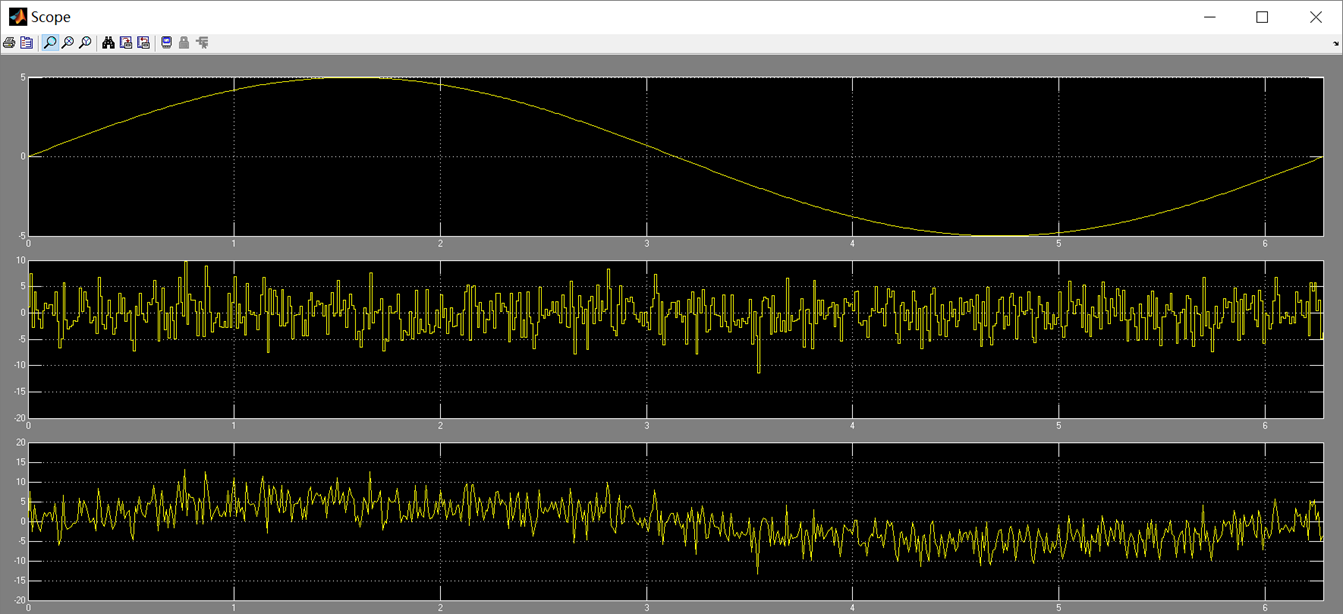
\includegraphics[scale=0.5]{matlab1}
\end{columns}
\end{frame}

\begin{frame}{简单二元信号波形检测---检测思路}
\begin{enumerate}
	\setlength{\itemsep}{.5cm}
	\item 首先,利用随机过程的正交级数展开,将随机过程用一组随机变量来表示;
	\item 然后,针对展开得到的随机变量,利用第三章的统计检测方法,构建贝叶斯检测表达式;
	\item 最后,令N趋向于无穷大, 利用展开系数与随机过程之间的表示关系,构建波形信号的检测表达式。
\end{enumerate}
\end{frame}

\begin{frame}{简单二元信号波形检测---检测思路}
\begin{columns}
\column{0.3\textwidth}
\begin{align*}
&x_k=\int_{0}^{T}x(t)f_k(t)dt\\
&s_k=\int_{0}^{T}s(t)f_k(t)dt\\
&n_k=\int_{0}^{T}n(t)f_k(t)dt\\
&x(t)=\lim\limits_{N\to\infty}^N\sum\limits_{k=1}^Nx_kf_k(t)\\
&\lambda(\bm{x}_N)=\frac{p(\bm{x}_N|H_1)}{p(\bm{x}_N|H_0)}\mathop{\gtrless}_{H_0}^{H_1}\eta\\
&\ln\lambda(x(t))\mathop{=}^{def}\lim\limits_{N\to\infty}[\lambda(\bm{x}_N)]\\
&l[x(t)]\mathop{\gtrless}_{H_0}^{H_1}\gamma
\end{align*}
\column{0.7\textwidth}
\centering
\tikzstyle{int}=[draw, fill=blue!20, minimum size=2em]
\begin{tikzpicture}[node distance=3.5cm,auto,>=latex']
\node [int] (a) {$x(t)$};
\node [int] (b) [right of=a] {$x_k$};
\node [int] (c) [right of=b] {$x_N$};
\node [int] (d) [below of=c] {$\frac{p(x_N|H_1)}{p(x_N|H_0)}\mathop{\gtrless}\limits_{H_0}^{H_1}\eta$};
\node [int] (e) [left of=d] {$l(x)\mathop{\gtrless}\limits_{H_0}^{H_1}\gamma$};
\path[->] (a) edge node {$\{f_k(t)\}$正交展开} (b);
\path[->] (b) edge node {前N项$x_k$构成$x_N$} (c);
\path[->] (c) edge [swap] node {贝叶斯检测} (d);
\path[->] (d) edge [swap] node {$N\to\infty$} (e);
\end{tikzpicture}
\end{columns}
\end{frame}

\begin{frame}{判决表达式---步骤1}
$H_0: x(t)=n(t)$\\
$H_1: x(t)=s(t)+n(t)$\\
\textbf{\textcolor{blue}{步骤1,选一组完备的正交函数集$\{f_k(t),k=1,2,\cdots \}$, 对接收信号进行正交级数展开,得到一组随机变量$x_k$}}\\
因为信号s(t)是确知信号,n(t)是均值为0的高斯白噪声,所以可以任选正交函数集$\{f_k(t)\}$
\begin{align*}
&x_k=\int_{0}^{T}x(t)f_k(t)dt &\qquad x(t)=\lim\limits_{N\to\infty}^N\sum\limits_{k=1}^Nx_kf_k(t)\\
&H_0: x_k=n_k,k=1,2,\dots &\qquad n_k=\int_{0}^{T}n(t)f_k(t)dt\\
&H_1: x_k=s_k+n_k,k=1,2,\dots &\qquad s_k=\int_{0}^{T}s(t)f_k(t)dt
\end{align*}
\end{frame}

\begin{frame}{判决表达式---步骤1}
\begin{itemize}
	\item 信号s(t)是确知信号,n(t)是均值为0,功率谱密度为$P_n(\omega)=N_0/2$的高斯白噪声;
	\item 无论在假设$H_1$下还是在假设$H_2$下,接收信号的$x(t)$都是高斯随机过程;
	\item 展开系数$x_k$是高斯随机过程的积分结果,因而$x_k$是高斯随机变量;
	\item 展开系数$x_k$之间是互不相关的,也是相互统计独立的;
	\item 高斯随机变量由均值和方差决定。由此求出两个假设下的概率密度函数$p(x_k|H_j),k=1,2,\dots;j=0,1$。
\end{itemize}
\end{frame}

\begin{frame}[shrink]{判决表达式---步骤1: 假设$H_0$下$x_k$的均值和方差}
\begin{align*}
H_0: x_k=n_k, \quad n_k=\int_{0}^{T}n(t)f_k(t)dt
\end{align*}
由于$n(t)$是均值为零的高斯白噪声
\begin{align*}
&E[n(t)]=0, \qquad E[n(t)n(u)]=r_n(t-u) =\frac{N_0}{2}\delta(t-u)=\frac{N_0}{2},(\delta(t-u)=1,t=u)
\end{align*}
$f_k(t)$是一组正交函数集$\implies\int_{0}^{T}f_j(t)f_k(t)dt=1,(j=k)$
\begin{align*}
E[x_k|H_0]&=E[n_k]=E\left[\int_{0}^{T}n(t)f_k(t)dt\right]=\int_{0}^{T}E[n(t)]f_k(t)dt=0\\
Var[x_k|H_0]&=E[n_k^2]=E\left[\int_{0}^{T}n(t)f_k(t)dt\int_{0}^{T}n(u)f_k(u)du\right]\\
&=\int_{0}^{T}f_k(t)\left\{\int_{0}^{T}E[n(t)n(u)]f_k(u)du\right\}dt=\int_{0}^{T}f_k(t)\left[\int_{0}^{T}\frac{N_0}{2}\delta(t-u)f_k(u)du\right]dt\\
&=\int_{0}^{T}f_k(t)\frac{N_0}{2}f_k(t)dt=\frac{N_0}{2}
\end{align*}
\end{frame}

\begin{frame}[shrink]{判决表达式---步骤1: 假设$H_1$下$x_k$的均值和方差}
\begin{align*}
H_1: x_k=s_k+n_k, \quad s_k=\int_{0}^{T}s(t)f_k(t)dt, \quad n_k=\int_{0}^{T}n(t)f_k(t)dt
\end{align*}
\begin{align*}
E[x_k|H_1]&=E[s_k+n_k]&\text{by }x_k=s_k+n_k \\
&=E(s_k)+E(n_k)&\text{by }E(n_k)=0 \\
&=E(s_k)=s_k&\text{(确知信号展开系数为确定量,其均值就是本身)}\\
Var[x_k|H_1]&=E[(x_k-E[x_k])^2]&\text{by }x_k=s_k+n_k,E[x_k]=s_k\\
&=E[(s_k+n_k-s_k)^2]&\\
&=E[n_k^2]=\frac{N_0}{2}&
\end{align*}
\end{frame}

\begin{frame}[shrink]{判决表达式---步骤1: 假设$H_0,H_1$下$x_k$的概率密度}
\begin{align*}
E[x_k|H_0]=0,   &\quad Var[x_k|H_1]=\frac{N_0}{2}\\
E[x_k|H_1]=s_k, &\quad Var[x_k|H_1]=\frac{N_0}{2}
\end{align*}
\begin{align*}
p(x_k|H_0)&=\left(\frac{1}{\pi N_0}\right)^{1/2}\exp\left(-\frac{x_k^2}{N_0}\right), k=1,2,\cdots\\
p(x_k|H_1)&=\left(\frac{1}{\pi N_0}\right)^{1/2}\exp\left(-\frac{(x_k^2-s_k)^2}{N_0}\right), k=1,2,\cdots
\end{align*}
\end{frame}

\begin{frame}[shrink]{判决表达式---步骤2}
\textbf{\textcolor{blue}{步骤2,利用前$N$项展开系数, 构建似然比检验。由于信道是加性高斯白噪声, 由卡亨南---洛维展开可知, 各展开系数是不相关的, 因而也是相互独立的。}}
\begin{align*}
p(\bm{x}_N|H_0)&=\prod_{k=1}^{N}p(x_k|H_0)=\prod_{k=1}^{N}\left(\frac{1}{\pi N_0}\right)^{1/2}\exp\left(-\frac{x_k^2}{N_0}\right)\\
p(\bm{x}_N|H_1)&=\prod_{k=1}^{N}p(x_k|H_1)=\prod_{k=1}^{N}\left(\frac{1}{\pi N_0}\right)^{1/2}\exp\left(-\frac{(x_k^2-s_k)^2}{N_0}\right)
\end{align*}
\[\bm{x}_N=(x_1,x_2,\cdots)^T\]		
\end{frame}

\begin{frame}[shrink]{判决表达式---步骤2: 似然比}
\begin{align*}
\lambda(\bm{x}_N)=\frac{p(\bm{x}_N|H_1)}{p(\bm{x}_N|H_0)}&\mathop{\gtrless}_{H_0}^{H_1}\eta\\
\frac{\prod\limits_{k=1}^{N}\left(\frac{1}{\pi N_0}\right)^{1/2}\exp\left(-\frac{x_k^2}{N_0}\right)}
{\prod\limits_{k=1}^{N}\left(\frac{1}{\pi N_0}\right)^{1/2}\exp\left(-\frac{(x_k^2-s_k)^2}{N_0}\right)}&\mathop{\gtrless}_{H_0}^{H_1}\eta
\end{align*}
化简,得到
\[\ln\lambda(\bm{x}_N)=\frac{p(\bm{x}_N|H_1)}{p(\bm{x}_N|H_0)}=\frac{2}{N_0}\sum\limits_{k=1}^{N}x_ks_k-\frac{1}{N_0}\sum\limits_{k=1}^{N}s_k^2\mathop{\gtrless}_{H_0}^{H_1}\ln\eta \]

\end{frame}

\begin{frame}[shrink]{判决表达式---步骤3}
\[\ln\lambda(\bm{x}_N)=\frac{p(\bm{x}_N|H_1)}{p(\bm{x}_N|H_0)}=\frac{2}{N_0}\sum\limits_{k=1}^{N}x_ks_k-\frac{1}{N_0}\sum\limits_{k=1}^{N}s_k^2\mathop{\gtrless}_{H_0}^{H_1}\ln\eta \]
\textbf{\textcolor{blue}{步骤3, 令$N\to\infty$, 将离散判决式变成连续形式}}
因为在两个假设下接收信号$x(t)(0\le t\le T)$的展开系数$x_k(k=1,2,\cdots)$是无穷多个,而离散形式判决式只是取前有限$N$项的结果,因此应对上式取$N\to\infty$的极限。
\[\ln\lambda(x(t))\mathop{=}^{def}\lim\limits_{N\to\infty}[\ln\lambda(\bm{x}_N)]=\lim\limits_{N\to\infty}\left(\frac{2}{N_0}\sum\limits_{k=1}^{N}x_ks_k-\frac{1}{N_0}\sum\limits_{k=1}^{N}s_k^2\right) \]
\[\ln\lambda(x(t))\mathop{\gtrless}_{H_0}^{H_1}\ln\eta \]
\[\ln\lambda(x(t))\mathop{=}^{def}\lim\limits_{N\to\infty}\left(\frac{2}{N_0}\sum\limits_{k=1}^{N}x_ks_k-\frac{1}{N_0}\sum\limits_{k=1}^{N}s_k^2\right)=
\frac{2}{N_0}\lim\limits_{N\to\infty}\sum\limits_{k=1}^{N}x_ks_k-\frac{1}{N_0}\lim\limits_{N\to\infty}\sum\limits_{k=1}^{N}s_k^2\mathop{\gtrless}_{H_0}^{H_1}\ln\eta \]
\end{frame}

\begin{frame}{判决表达式---步骤3: 推导(1)}
\[\ln\lambda(x(t))\mathop{=}^{def}
\frac{2}{N_0}\lim\limits_{N\to\infty}\sum\limits_{k=1}^{N}x_ks_k-\frac{1}{N_0}\lim\limits_{N\to\infty}\sum\limits_{k=1}^{N}s_k^2\mathop{\gtrless}_{H_0}^{H_1}\ln\eta \]
\begin{align*}
\lim\limits_{N\to\infty}\sum\limits_{k=1}^{N}x_ks_k&=\left[\lim\limits_{N\to\infty}\sum\limits_{k=1}^{N}x_k\right]s_k &&\text{by }s_k=\int_{0}^{T}s(t)f_k(t)dt \\
&=\left[\lim\limits_{N\to\infty}\sum\limits_{k=1}^{N}x_k\right]\int_{0}^{T}s(t)f_k(t)dt\\
&=\int_{0}^{T}s(t)\left[\lim\limits_{N\to\infty}\sum\limits_{k=1}^{N}x_kf_k(t)\right]dt &&\text{by }x(t)=\lim\limits_{N\to\infty}\sum\limits_{k=1}^Nx_kf_k(t)\\
&=\int_{0}^{T}s(t)x(t)dt
\end{align*}
\end{frame}

\begin{frame}{判决表达式---步骤3: 推导(2)}
\[\ln\lambda(x(t))\mathop{=}^{def}
\frac{2}{N_0}\lim\limits_{N\to\infty}\sum\limits_{k=1}^{N}x_ks_k-\frac{1}{N_0}\lim\limits_{N\to\infty}\sum\limits_{k=1}^{N}s_k^2\mathop{\gtrless}_{H_0}^{H_1}\ln\eta \]
\begin{align*}
\lim\limits_{N\to\infty}\sum\limits_{k=1}^{N}s_k^2&=\left[\lim\limits_{N\to\infty}\sum\limits_{k=1}^{N}s_k\right]s_k &&\text{by }s_k=\int_{0}^{T}s(t)f_k(t)dt \\
&=\left[\lim\limits_{N\to\infty}\sum\limits_{k=1}^{N}s_k\right]\int_{0}^{T}s(t)f_k(t)dt\\
&=\int_{0}^{T}s(t)\left[\lim\limits_{N\to\infty}\sum\limits_{k=1}^{N}s_kf_k(t)\right]dt &&\text{by }s(t)=\lim\limits_{N\to\infty}\sum\limits_{k=1}^Ns_kf_k(t)\\
&=\int_{0}^{T}s(t)s(t)dt=\int_{0}^{T}s^2(t)dt &&\text{by }E_s=\int_{0}^{T}s^2(t)dt\\
&=E_s
\end{align*}
\end{frame}

\begin{frame}{判决表达式---步骤3: 推导(3)}
\[\ln\lambda(x(t))\mathop{=}^{def}
\frac{2}{N_0}\lim\limits_{N\to\infty}\sum\limits_{k=1}^{N}x_ks_k-\frac{1}{N_0}\lim\limits_{N\to\infty}\sum\limits_{k=1}^{N}s_k^2\mathop{\gtrless}_{H_0}^{H_1}\ln\eta \]
\begin{align*}
\lim\limits_{N\to\infty}\sum\limits_{k=1}^{N}x_ks_k=\int_{0}^{T}s(t)x(t)dt, \qquad \lim\limits_{N\to\infty}\sum\limits_{k=1}^{N}s_k^2=E_s
\end{align*}
判决表达式:
\[\ln\lambda(x(t))\mathop{=}^{def}\frac{2}{N_0}\int_{0}^{T}s(t)x(t)dt-\frac{E_s}{N_0}\mathop{\gtrless}_{H_0}^{H_1}\ln\eta\]
化简为:
\[l[x(t)]\mathop{=}^{def}\int_{0}^{T}s(t)x(t)dt\mathop{\gtrless}_{H_0}^{H_1}\frac{N_0}{2}\ln\eta+\frac{E_s}{2}\mathop{=}^{def}\gamma\]
\end{frame}

\begin{frame}{简单二元信号波形的检测---检测系统结构}
\begin{columns}
	\column{0.4\textwidth}
	\small
	\textbf{检测系统的结构}:最佳检测系统(又称最佳接收机)的结构,根据信号最佳检测的判决表达式来设计。\\
	检测统计量$l[x(t)$是由接收信号$x(t)$与确知信号$s(t)$经相关运算得到的,所以这种结构称为\textbf{相关检测系统},是由互相关器和判决器实现。\\
	白噪声下t=T时刻匹配滤波器输出信号与相关器输出信号式相等的。所以也可以用匹配滤波器和判决器来实现。
	\column{0.6\textwidth}
	\[l[x(t)]\mathop{=}^{def}\int_{0}^{T}s(t)x(t)dt\mathop{\gtrless}_{H_0}^{H_1}\frac{N_0}{2}\ln\eta+\frac{E_s}{2}\mathop{=}^{def}\gamma\]
	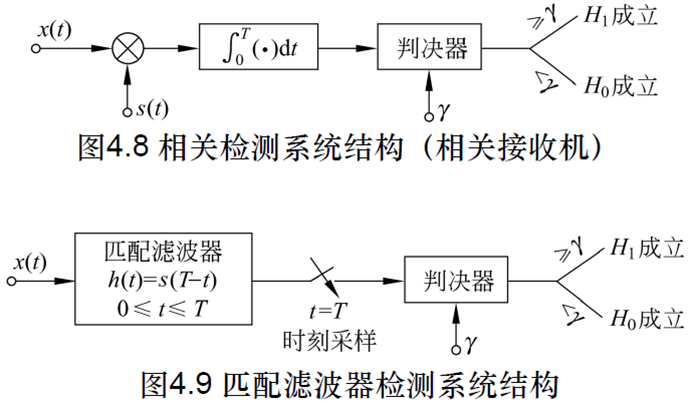
\includegraphics[scale=0.4]{4-8}
\end{columns}
\end{frame}

\begin{frame}[shrink]
\begin{align*}
\text{信源发送信号: } &s(t)=\sin(t),0 \le t\le T\\
\text{接收信号: } &x(t)=s(t)+n(t), 0\le t\le T
\end{align*}
%\vspace{0.5cm}
\centering
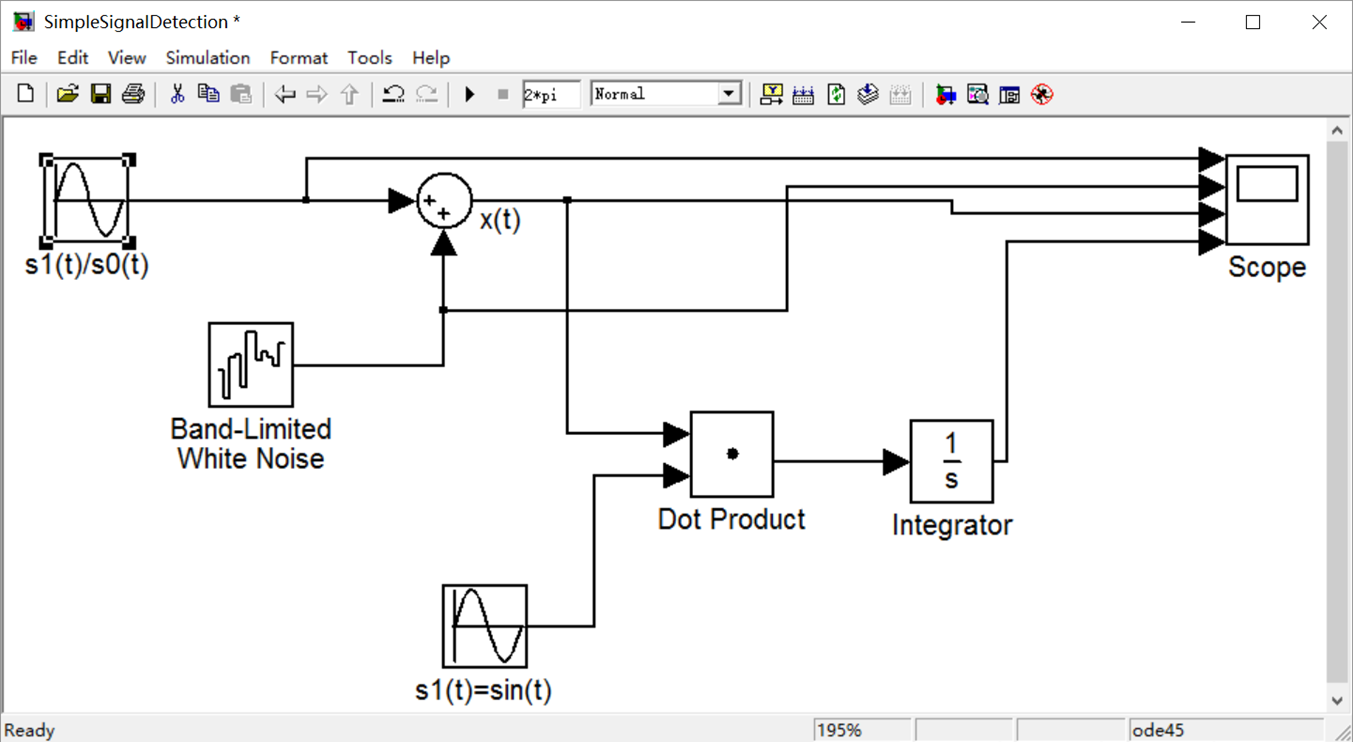
\includegraphics[scale=0.6]{matlab2}
\end{frame}

\begin{frame}[shrink]
\begin{align*}
\text{信源发送信号: } &s(t)=5\sin(t),0 \le t\le T\\
\text{接收信号: } &x(t)=s(t)+n(t), 0\le t\le T
\end{align*}
%\vspace{0.5cm}
\begin{columns}%[T]
	\column{0.05\textwidth}
	~\\
	\vspace{0.2cm}
	$s(t)$\\
	\vspace{0.5cm}
	$n(t)$\\
	\vspace{0.5cm}
	$H_0$\\
	\vspace{0.5cm}
	$H_1$\\
	\column{0.95\textwidth}
	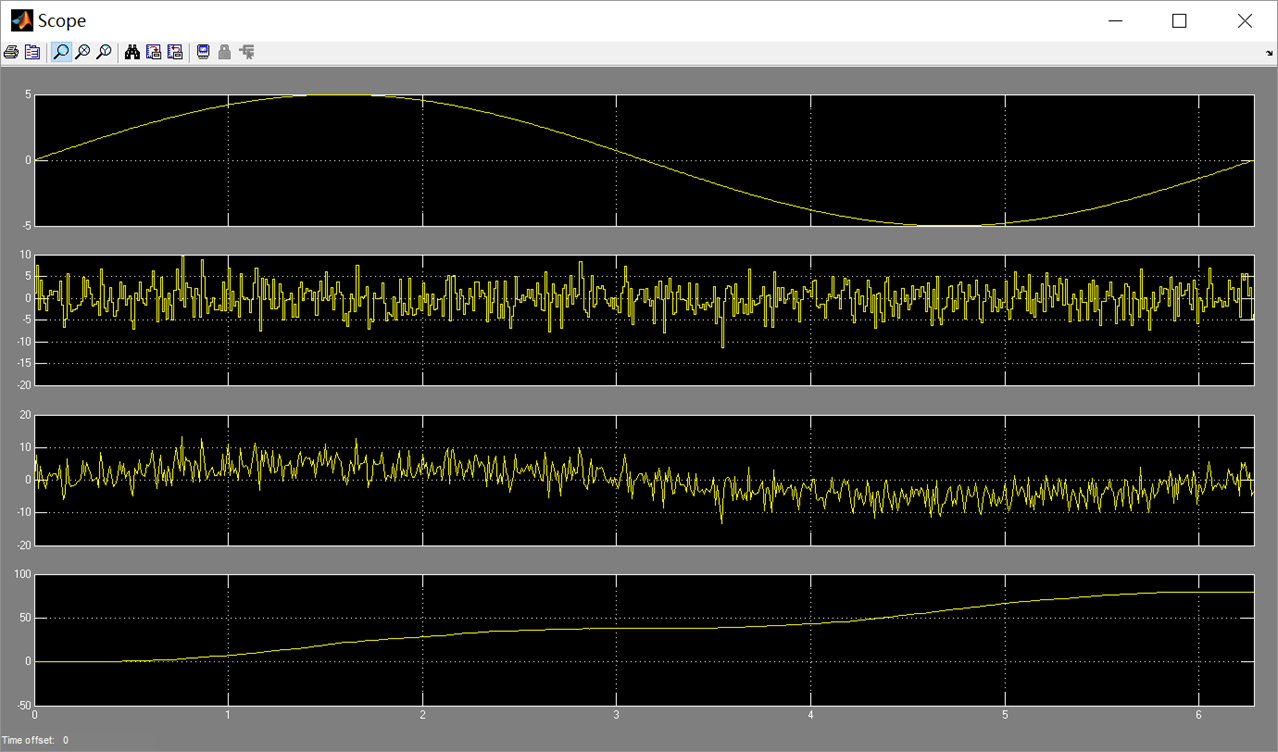
\includegraphics[scale=0.45]{matlab3}
\end{columns}
\end{frame}

\begin{frame}[shrink]
\begin{align*}
\text{信源发送信号: } &s(t)=0,0 \le t\le T\\
\text{接收信号: } &x(t)=s(t)+n(t), 0\le t\le T
\end{align*}
%\vspace{0.5cm}
\begin{columns}%[T]
	\column{0.05\textwidth}
	~\\
	\vspace{0.2cm}
	$s(t)$\\
	\vspace{0.5cm}
	$n(t)$\\
	\vspace{0.5cm}
	$H_0$\\
	\vspace{0.5cm}
	$H_1$\\
	\column{0.95\textwidth}
	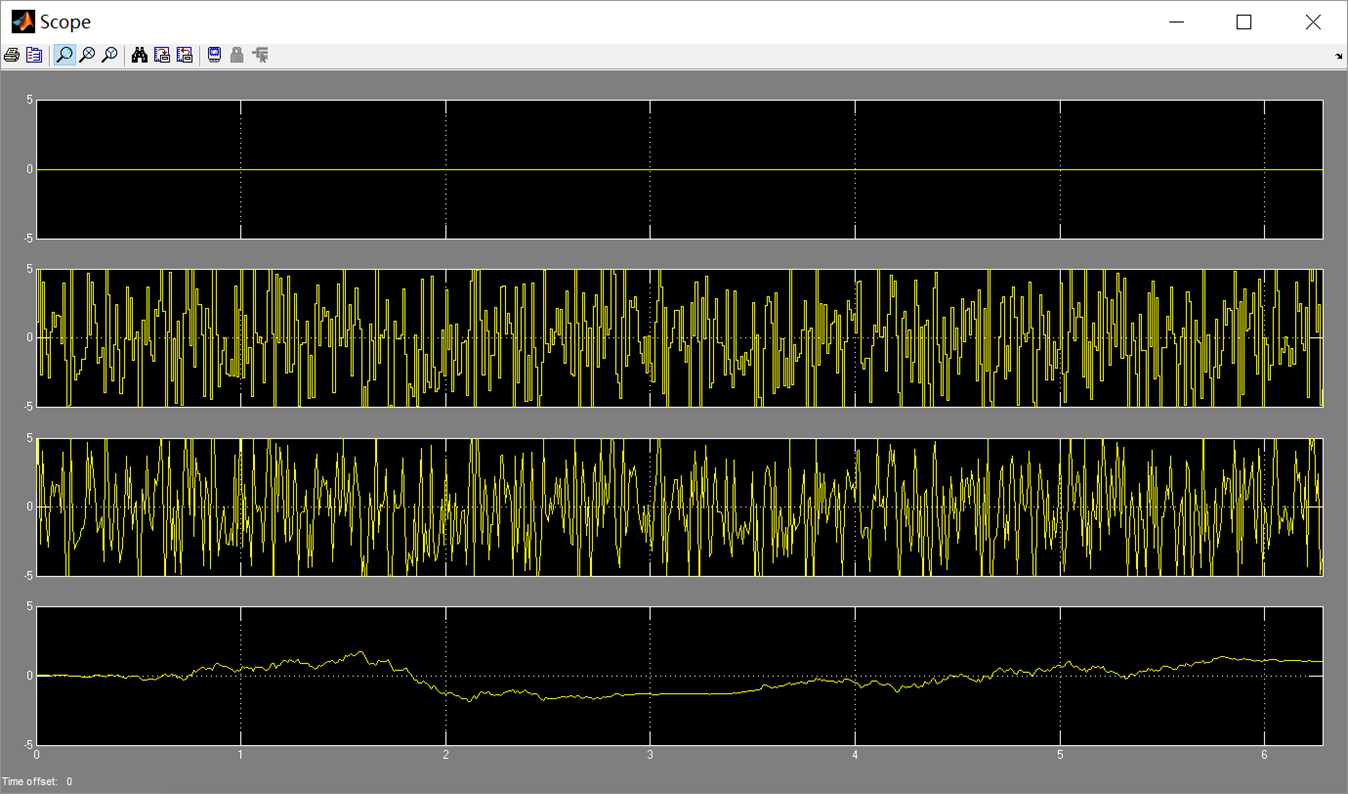
\includegraphics[scale=0.4]{matlab4}
\end{columns}
\end{frame}
\begin{frame}{简单二元信号波形检测---步骤归纳}
\begin{enumerate}
	\setlength{\itemsep}{.5cm}
	\item 首先,利用随机过程的正交级数展开,将随机过程用一组随机变量来表示;
	\item 然后,针对展开得到的随机变量,利用第三章的统计检测方法,构建贝叶斯检测表达式;
	\item 最后,令N趋向于无穷大, 利用展开系数与随机过程之间的表示关系,构建波形信号的检测表达式。
\end{enumerate}
\[ l[x(t)]\mathop{=}^{def}\int_{0}^{T}s(t)x(t)dt\mathop{\gtrless}_{H_0}^{H_1}\frac{N_0}{2}\ln\eta+\frac{E_s}{2}\mathop{=}^{def}\gamma \]
\end{frame}

\begin{frame}{简单二元信号波形检测---步骤归纳}
\begin{columns}
\column{0.3\textwidth}
\begin{align*}
&x_k=\int_{0}^{T}x(t)f_k(t)dt\\
&s_k=\int_{0}^{T}s(t)f_k(t)dt\\
&n_k=\int_{0}^{T}n(t)f_k(t)dt\\
&x(t)=\lim\limits_{N\to\infty}^N\sum\limits_{k=1}^Nx_kf_k(t)\\
&\lambda(\bm{x}_N)=\frac{p(\bm{x}_N|H_1)}{p(\bm{x}_N|H_0)}\mathop{\gtrless}_{H_0}^{H_1}\eta\\
&\ln\lambda(x(t))\mathop{=}^{def}\lim\limits_{N\to\infty}[\lambda(\bm{x}_N)]\\
&l[x(t)]\mathop{\gtrless}_{H_0}^{H_1}\gamma
\end{align*}
\column{0.7\textwidth}
\centering
\tikzstyle{int}=[draw, fill=blue!20, minimum size=2em]
\begin{tikzpicture}[node distance=3.5cm,auto,>=latex']
\node [int] (a) {$x(t)$};
\node [int] (b) [right of=a] {$x_k$};
\node [int] (c) [right of=b] {$x_N$};
\node [int] (d) [below of=c] {$\frac{p(x_N|H_1)}{p(x_N|H_0)}\mathop{\gtrless}\limits_{H_0}^{H_1}\eta$};
\node [int] (e) [left of=d] {$l(x)\mathop{\gtrless}\limits_{H_0}^{H_1}\gamma$};
\path[->] (a) edge node {$\{f_k(t)\}$正交展开} (b);
\path[->] (b) edge node {前N项$x_k$构成$x_N$} (c);
\path[->] (c) edge [swap] node {贝叶斯检测} (d);
\path[->] (d) edge [swap] node {$N\to\infty$} (e);
\end{tikzpicture}
\[ l[x(t)]\mathop{=}^{def}\int_{0}^{T}s(t)x(t)dt\mathop{\gtrless}_{H_0}^{H_1}\frac{N_0}{2}\ln\eta+\frac{E_s}{2}\mathop{=}^{def}\gamma \]
\end{columns}
\end{frame}

\begin{frame}{简单二元信号波形检测要点}
\begin{columns}
	\column{0.4\textwidth}
	$H_0: x(t)=n(t)$\\
	$H_1: x(t)=s(t)+n(t)$\\
	$x(t)=\lim\limits_{N\to\infty}^N\sum\limits_{k=1}^Nx_kf_k(t)$\\
	$x_k=\int_{0}^{T}x(t)f_k(t)dt, k=1,2,\dots$\\
	$s_k=\int_{0}^{T}s(t)f_k(t)dt, k=1,2,\dots$\\
	$n_k=\int_{0}^{T}n(t)f_k(t)dt, k=1,2,\dots$\\
	$H_0: x_k=n_k,k=1,2,\dots$\\
	$H_1: x_k=s_k+n_k,k=1,2,\dots$
	\[ \int_{0}^{T}s(t)x(t)dt\mathop{\gtrless}_{H_0}^{H_1}\frac{N_0}{2}\ln\eta+\frac{E_s}{2} \]
	\column{0.6\textwidth}
	\begin{itemize}
		\item 信号s(t)是确知信号,n(t)是均值为0,功率谱密度为$P_n(\omega)=N_0/2$的高斯白噪声;
		\item 无论在假设$H_1$下还是在假设$H_2$下,接收信号的$x(t)$都是高斯随机过程;
		\item 展开系数$x_k$是高斯随机过程的积分结果,因而$x_k$是高斯随机变量;
		\item 展开系数$x_k$之间是互不相关的,也是相互统计独立的;
		\item 高斯随机变量由均值和方差决定。由此求出两个假设下的概率密度函数$p(x_k|H_j),k=1,2,\dots;j=0,1$。
	\end{itemize}
\end{columns}
\end{frame}

\begin{frame}{$x_k,s_k,n_k$之间的关系}
\begin{block}{$x_k,s_k,n_k$之间的关系}
	\[x(t)=s(t)+n(t); \quad x_k=s_k+n_k \]
	随机变量$x(t)$展开系数$x_k$=确知信号$s(t)$展开系数$s_k$+噪声$n(t)$展开系数$n_k$
\end{block}
\begin{align*}
x_k&=\int_{0}^{T}f_k(t)x(t)dt\\
&=\int_{0}^{T}f_k(t)(s(t)+n(t))dt\\
&=\int_{0}^{T}f_k(t)s(t)dt+\int_{0}^{T}f_k(t)n(t))dt\\
&=s_k+n_k
\end{align*}
\end{frame}

\section{检测系统性能分析}

\begin{frame}{简单二元信号波形检测-检测性能(1)}
$H_0: x(t)=n(t), \quad H_1: x(t)=s(t)+n(t)$\\
\textbf{判决表达式:}
\[l[x(t)]\mathop{=}^{def}\int_{0}^{T}x(t)s(t)dt\mathop{\gtrless}_{H_0}^{H_1}\frac{N_0}{2}\ln\eta+\frac{E_s}{2}\mathop{=}^{def}\gamma \]
检验统计量$l[x(t)]$无论在假设$H_0$下,还是在假设$H_1$下,都是由高斯随机过程$x(t)s(t)(0\le t\le T)$经积分得到的,所以\bm{$l[x(t)]$}\textbf{是高斯随机变量}。
\begin{enumerate}
	\item 求出检验统计量$l[x(t)]$在两个假设下的均值$E(l|H_j)$和方差$Var(l|H_j),j=0,1$;
	\item 求各种判决概率$P(H_i|H_j),i,j=0,1$;\\
	简单二元信号检测与雷达信号检测相对应:$P(H_1|H_0)\mathop{=}\limits^{def}P_F$(称为虚警概率),$P(H_1|H_1)\mathop{=}\limits^{def}P_D$(称为检测概率)
	\item 计算检测性能。
\end{enumerate}
\end{frame}

\begin{frame}[shrink]{简单二元信号波形检测-检测性能(2)}
\begin{enumerate}[1]
\item 定义统计量:
\[l[x(t)]\mathop{=}\limits^{def}\int_{0}^{T}x(t)s(t)dt \]
\item 假设$H_0,H_1$下检验统计量$l[x(t)]$的均值和方差分别为
\begin{align*}
E[l|H_0]&=E\left[\int_{0}^{T}x(t)s(t)dt|H_0\right]=E\left[\int_{0}^{T}n(t)s(t)dt\right]=0\\ 
Var[l|H_0]&=E[((l|H_0)-E(l|H_0))^2]=\frac{N_0}{2}E_s\\
E[l|H_1]&=E\left[\int_{0}^{T}x(t)s(t)dt|H_1\right]=E\left[\int_{0}^{T}(s(t)+n(t))s(t)dt\right]=E_s\\
Var[l|H_1]&=E[((l|H_1)-E(l|H_1))^2]=\frac{N_0}{2}E_s
\end{align*}
\item 假设$H_0,H_1$下服从高斯分布的检验统计量$l[x(t)]$的概率密度函数分别为\\
\[p(l|H_0)=\left(\frac{1}{\pi N_0E_s}\right)^{1/2}\exp\left(-\frac{l^2}{N_0E_s}\right),\quad p(l|H_1)=\left(\frac{1}{\pi N_0E_s}\right)^{1/2}\exp\left(-\frac{(l-E_s)^2}{N_0E_s}\right)\]
\end{enumerate}
\end{frame}

\begin{frame}[shrink]{简单二元信号波形检测-检测性能(3)}
\begin{enumerate}
\setcounter{enumi}{3} 
\item 求各种判决概率$P(H_i|H_j),i,j=0,1$
\begin{columns}
\column{0.6\textwidth}
\begin{align*}
&\text{虚警概率:} P(H_1|H_0)\mathop{=}\limits^{def}P_F=Q\left[\frac{\ln\eta}{d}+\frac{d}{2}\right]\\ 
&\text{检测概率:} P(H_1|H_1)\mathop{=}\limits^{def}P_D=Q\left[\frac{\ln\eta}{d}-\frac{d}{2}\right]\\
&P(H_0|H_1)=1-P(H_1|H_1)=1-Q\left[\frac{\ln\eta}{d}-\frac{d}{2}\right]\\
&P(H_0|H_0)=1-P(H_1|H_0)=1-Q\left[\frac{\ln\eta}{d}+\frac{d}{2}\right]
\end{align*}
\column{0.4\textwidth}
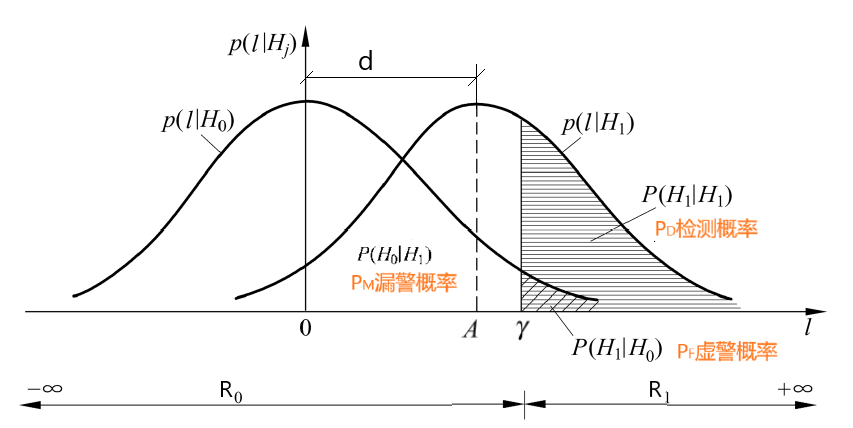
\includegraphics[scale=0.3]{R0R1}
\end{columns}
\[d^2\mathop{=}\limits^{def}\frac{(E(l|H_1)-E(l|H_0))^2}{Var(l|H_0)}=\frac{2E_s}{N_0} \quad \text{偏移系数$d^2$表示功率信噪比}\]
\end{enumerate}
\begin{block}{结论}
对简单二元信号来讲,只要保持确知信号$s(t)$的能量不变,信号波形可以任意设计,检测性能不发生变化。
\end{block}
\end{frame}

\begin{frame}[shrink]{计算$E[l|H_0]$和$Var[l|H_0]$}
\begin{align*}
&l[x(t)]\mathop{=}\limits^{def}\int_{0}^{T}x(t)s(t)dt,\quad E_s=\int_{0}^{T}s^2(t)dt,\quad H_0:x(t)=n(t), \quad E[n(t)]=0\\
&E[n(t)n(u)]=r_n(t-u)=\frac{N_0}{2}\delta(t-u)=\frac{N_0}{2},(t=u,\delta(t-u)=1)
\end{align*}
\begin{align*}
E[l|H_0]&=E\left[\int_{0}^{T}x(t)s(t)dt|H_0\right]=E\left[\int_{0}^{T}n(t)s(t)dt\right]=\int_{0}^{T}E[n(t)]s(t)dt=0\\
Var[l|H_0]&=E[((l|H_0)-E(l|H_0))^2]=E[(l|H_0)^2]=E\left[\left(\int_{0}^{T}x(t)s(t)dt\right)^2\right]\\
&=E\left[\int_{0}^{T}n(t)s(t)dt\int_{0}^{T}n(t)s(t)dt\right]=E\left[\int_{0}^{T}n(t)s(t)dt\int_{0}^{T}n(u)s(u)du\right]\\
&=\int_{0}^{T}s(t)\left\{\int_{0}^{T}E[n(u)n(t)]s(u)du\right\}dt=\int_{0}^{T}s(t)\left[\int_{0}^{T}\frac{N_0}{2}\delta(t-u)s(u)du\right]dt\\
&=\frac{N_0}{2}\int_{0}^{T}s(t)\left(\int_{0}^{T}s(u)du\right)dt=\frac{N_0}{2}\int_{0}^{T}s^2(t)dt=\frac{N_0}{2}E_s
\end{align*}
\end{frame}

\begin{frame}{计算$p(l|H_0)$}
\[ E[l|H_0]=0,\quad Var[l|H_0]=\frac{N_0}{2}E_s \]
\begin{align*}
p(l|H_0)&=\left(\frac{1}{2\pi Var[l|H_0]}\right)^{1/2}\exp\left(-\frac{(l-E[l|H_0])^2}{2Var[l|H_0]}\right)\\
&=\left(\frac{1}{\pi N_0E_s}\right)^{1/2}\exp\left(-\frac{l^2}{N_0E_s}\right)
\end{align*}
\end{frame}

\begin{frame}[shrink]{计算$E[l|H_1]$}
\begin{align*}
&l[x(t)]\mathop{=}\limits^{def}\int_{0}^{T}x(t)s(t)dt,\quad E_s=\int_{0}^{T}s^2(t)dt,\quad H_1:x(t)=s(t)+n(t), \quad E[n(t)]=0
\end{align*}
\begin{align*}
E[l|H_1]&=E\left[\int_{0}^{T}x(t)s(t)dt|H_1\right] &&\text{by }H_1: x(t)=s(t)+n(t)\\
&=E\left[\int_{0}^{T}(s(t)+n(t))s(t)dt\right]\\
&=E\left[\int_{0}^{T}s^2(t)dt\right]+\int_{0}^{T}E[n(t)]s(t)dt &&\text{by } E[n(t)]=0 \\
&=E\left[\int_{0}^{T}s^2(t)dt\right] &&\text{by } E_s=\int_{0}^{T}s^2(t)dt\\
&=E_s
\end{align*}
\end{frame}

\begin{frame}[shrink]{计算$Var[l|H_1]$}
\begin{align*}
&l[x(t)]\mathop{=}\limits^{def}\int_{0}^{T}x(t)s(t)dt,\quad E_s=\int_{0}^{T}s^2(t)dt,\quad H_1:x(t)=s(t)+n(t), \quad E[n(t)]=0\\
&E[n(t)n(u)]=r_n(t-u)=\frac{N_0}{2}\delta(t-u)=\frac{N_0}{2},(t=u,\delta(t-u)=1)
\end{align*}
\begin{align*}
Var[l|H_1]&=E[((l|H_1)-E(l|H_1))^2]=E\left[\left(\int_{0}^{T}(s(t)+n(t))s(t)dt-E_s\right)^2\right]\\
&=E\left[\left(\int_{0}^{T}(s^2(t)dt+\int_{0}^{T}n(t)s(t)dt-E_s\right)^2\right]=E\left[\left(\int_{0}^{T}n(t)s(t)dt\right)^2\right]\\
&=E\left[\int_{0}^{T}n(t)s(t)dt\int_{0}^{T}n(t)s(t)dt\right]=E\left[\int_{0}^{T}n(t)s(t)dt\int_{0}^{T}n(u)s(u)du\right]\\
&=\int_{0}^{T}s(t)\left\{\int_{0}^{T}E[n(u)n(t)]s(u)du\right\}dt=\int_{0}^{T}s(t)\left[\int_{0}^{T}\frac{N_0}{2}\delta(t-u)s(u)du\right]dt\\
&=\frac{N_0}{2}\int_{0}^{T}s(t)\left(\int_{0}^{T}s(u)du\right)dt=\frac{N_0}{2}\int_{0}^{T}s^2(t)dt=\frac{N_0}{2}E_s
\end{align*}
\end{frame}

\begin{frame}{计算$p(l|H_1)$}
\[ E[l|H_1]=E_s,\quad Var[l|H_1]=\frac{N_0}{2}E_s \]
\begin{align*}
	p(l|H_1)&=\left(\frac{1}{2\pi Var[l|H_1]}\right)^{1/2}\exp\left(-\frac{(l-E[l|H_1])^2}{2Var[l|H_1]}\right)\\
	&=\left(\frac{1}{\pi N_0E_s}\right)^{1/2}\exp\left(-\frac{(l-E_s)^2}{N_0E_s}\right)
\end{align*}
\end{frame}

\begin{frame}[shrink]{计算$P(H_1|H_0)$}
\begin{align*}
p(l|H_0)&=\left(\frac{1}{\pi N_0E_s}\right)^{1/2}\exp\left(-\frac{l^2}{N_0E_s}\right)\\
P(H_1|H_0)&\mathop{=}^{def}P_F=\int_{\gamma}^{\infty}p(l|H_0)dl\qquad \implies&& Q(x)=\int_{x}^{\infty}\left(\frac{1}{2\pi}\right)^{1/2}\exp\left(-\frac{u^2}{2}\right)du\\
&=\int_{\gamma}^{\infty}\left(\frac{1}{\pi N_0E_s}\right)^{1/2}\exp\left(-\frac{l^2}{N_0E_s}\right)dl&&\text{by }l=u\sqrt{N_0E_s/2}\\
&=\int_{\frac{\gamma}{\sqrt{N_0E_s/2}}}^{\infty}\left(\frac{1}{2\pi}\right)^{1/2}\exp\left(-\frac{u^2}{2}\right)du\\
&=Q\left[\frac{\gamma}{\sqrt{N_0E_s/2}}\right]&&\text{by }\gamma=\frac{N_0}{2}\ln\eta+\frac{E_s}{2}\\
&=Q\left[\frac{\frac{N_0}{2}\ln\eta+\frac{E_s}{2}}{\sqrt{N_0E_s/2}}\right]&&\text{by }d^2=\frac{2E_s}{N_0}\quad \text{偏移系数$d^2$表示功率信噪比。}\\
&=Q\left[\frac{\ln\eta}{d}+\frac{d}{2}\right] 
\end{align*}
\end{frame}

\begin{frame}[shrink]{计算$P(H_0|H_1)$}
\begin{align*}
p(l|H_1)&=\left(\frac{1}{\pi N_0E_s}\right)^{1/2}\exp\left(-\frac{(l-E_s)^2}{N_0E_s}\right)\\
P(H_1|H_1)&\mathop{=}^{def}P_D=\int_{\gamma}^{\infty}p(l|H_1)dl\qquad \implies&& Q(x)=\int_{x}^{\infty}\left(\frac{1}{2\pi}\right)^{1/2}\exp\left(-\frac{u^2}{2}\right)du\\
&=\int_{\gamma}^{\infty}\left(\frac{1}{\pi N_0E_s}\right)^{1/2}\exp\left(-\frac{(l-E_s)^2}{N_0E_s}\right)dl&&\text{by }l=u\sqrt{N_0E_s/2}+E_s\\
&=\int_{\frac{\gamma-E_s}{\sqrt{N_0E_s/2}}}^{\infty}\left(\frac{1}{2\pi}\right)^{1/2}\exp\left(-\frac{u^2}{2}\right)du\\
&=Q\left[\frac{\gamma-E_s}{\sqrt{N_0E_s/2}}\right]&&\text{by }\gamma=\frac{N_0}{2}\ln\eta+\frac{E_s}{2}\\
&=Q\left[\frac{\frac{N_0}{2}\ln\eta-\frac{E_s}{2}}{\sqrt{N_0E_s/2}}\right]&&\text{by }d^2=\frac{2E_s}{N_0}\quad \text{偏移系数$d^2$表示功率信噪比。}\\
&=Q\left[\frac{\ln\eta}{d}-\frac{d}{2}\right]
\end{align*}
\end{frame}
